
\subsection*{2. 解析函数与泰勒级数}

级数的一致收敛性可用于解决级数所表示的函数的微分与积分问题，所以首先要说明什么是复变量函数 $f(z)$ 在一点 $z_0$ 的导数。这时的导数与微分等概念形式上的与实变量函数无异，但是实质上大不相同。关于导数，我们仍定义
\begin{equation}
 f'(z_0)=\lim_{h\to0}\frac{f(z_0+h)-f(z_0)}{h}
 =\lim_{z\to z_0}\frac{f(z)-f(z_0)}{z-z_0}.
 \tag{10}
\end{equation}
这里 $h$ 是一个非 $0$ 复数，$z=z_0+h$。这样定义以后，实变量函数导数的基本性质，特别如莱布尼茨性质、复合函数导数的计算等都与实变量情况一样。$f$ 在 $z_0$ 点的微分仍定义为一个线性映射 $A:\mathbb C\to\mathbb C$ 使
\begin{equation}
 f(z_0+h)-f(z_0)=Ah+o(h).
 \tag{11}
\end{equation}
$A$ 就是“乘以 $f'(z_0)$”。在通常的教本上是把 $Ah$ 即 $\Delta f$ 之线性部分称为微分 $(df)(z_0)$ 的，而我们现在则用 $(df)(z_0)$ 表示一个线性映射，它作用在 $h$ 上的结果则是古典意义下的微分：
\[
 (df)(z_0)\cdot h=\text{古典意义下的微分}
 =f'(z_0)\,dz,\qquad dz=h.
\]
因为这一切与前面讲的没有区别，我们就不再重复。问题是如何求 $f'(z_0)$。由于至今我们还没有定义过多少具体的函数，如何计算导数就成了问题。但有两个非常重要的导数完全可用初等方法算出，一个是对非负整数 $k$，$(z^k)'=kz^{k-1}$。事实上，利用二项式定理，
\[
 (z^k)'=\lim_{h\to0}\frac1h\bigl[(z+h)^k-z^k\bigr]
 =\lim_{h\to0}\left(kz^{k-1}+\frac1{2!}k(k-1)z^{k-2}h+\cdots\right)
 =kz^{k-1}.
\]
另一个是
\[
 \left(\frac1z\right)'=-\frac1{z^2}.
\]
事实上
\[
 \left(\frac1z\right)'=\lim_{h\to0}\left(\frac1{z+h}-\frac1z\right)\bigg/h
 =\lim_{h\to0}\frac{-h}{z(z+h)}\cdot\frac1h
 =-\frac1{z^2}.
\]
此式当然只在 $z\ne0$ 时成立。类似地还有
\[
 \left(\frac1{z^k}\right)'=-\frac{k}{z^{k+1}}.
\]

由此，如果允许对幂级数(3)逐项求导，则应有
\[
 f'(z)=\sum_{n=0}^{\infty}na_nz^{n-1}.
\]
18世纪中，拉格朗日就认为可以用这样的方法来定义任意函数的导数，而完全用不着无穷小等概念。拉格朗日称此为纯粹“代数的方法”。这当然只是一个幻想，因为其中涉及无穷级数的逐项求导问题。这是一个困难的问题，通常微积分教本中关于这个问题的结果也有点怪，例如说，设某区间 $I$ 上的级数 $\sum_{n=0}^{\infty}f_n(x)$ 在 $x_0\in I$ 处收敛，且 $\sum_{n=0}^{\infty}\dfrac d{dx}f_n(x)$ 在 $I$ 上一致收敛，则原级数必可逐项求导：
\[
 \frac d{dx}\sum_{n=0}^{\infty}f_n(x)=\sum_{n=0}^{\infty}\frac d{dx}f_n(x).
\]
其所以如此是因为级数的逐项求导的问题被化成了 $\sum_{n=0}^{\infty}\dfrac d{dx}f_n(x)$ 的逐项求积（实际上是求原函数）。但是对幂级数(3)，则定理1给了我们十分自然的结果：

\noindent\textbf{定理3}\quad 若幂级数(3)之收敛半径为 $R>0$，其和为 $f(z)$，则
\begin{equation}
 f'(z)=\sum_{n=0}^{\infty}na_nz^{n-1},
 \tag{12}
\end{equation}
且收敛半径不变。

\noindent\textbf{证}\quad 先证(12)之收敛半径仍为 $R$。事实上
\[
\begin{aligned}
 \overline{\lim}_{n\to\infty}\sqrt[n-1]{|na_n|}
 &=\lim_{n\to\infty}\sqrt[n-1]{n}\;
   \overline{\lim}_{n\to\infty}\sqrt[n-1]{|a_n|}\\
 &=\lim_{n\to\infty}\sqrt[n-1]{n}
   \left(\overline{\lim}_{n\to\infty}\sqrt[n]{|a_n|}\right)^{\frac n{n-1}}.
\end{aligned}
\]
但是很容易看到 $\lim_{n\to\infty}\sqrt[n-1]{n}=1$。这是因为 $\sqrt[n-1]{n}>1$，故可写为
\[
 \sqrt[n-1]{n}=n^{\frac1{n-1}}=1+\alpha_n,\qquad \alpha_n>0.
\]
从而由二项式定理，
\[
 n=(1+\alpha_n)^{n-1}>1+\frac12(n-1)(n-2)\alpha_n^2,
\]
因此
\[
 0<\alpha_n^2<\frac{n-1}{\frac12(n-1)(n-2)}\to0.
\]
又利用求上极限问题可以化为求某个子序列的极限问题（我们不妨设 $|a_n|$ 就是这个子序列）又知
\[
 \overline{\lim}_{n\to\infty}\left(\sqrt[n]{|a_n|}\right)^{\frac n{n-1}}
 =\left(\lim_{n\to\infty}\sqrt[n]{|a_n|}\right)^{\lim\frac n{n-1}}
 =\overline{\lim}_{n\to\infty}\sqrt[n]{|a_n|}=\frac1R.
\]
所以级数(12)之收敛半径不变。

再证(12)之和为 $f'(z)$。设(12)之和为 $f_1(z)$，它也定义在 $|z|<R$ 上。又记(3)之部分和及余项分别为 $S_N(z)$ 与 $R_N(z)$：
\[
 S_N(z)=\sum_{n=0}^{N-1}a_nz^n,\qquad R_N(z)=\sum_{n=N}^{\infty}a_nz^n.
\]
对收敛圆 $|z|<R$ 内任一点 $z_0$（$|z_0|<R$ 是自然的，而且还可以找到正数 $\rho$ 使 $|z_0|<\rho<R$）考虑
\[
\begin{aligned}
 \frac{f(z)-f(z_0)}{z-z_0}-f_1(z_0)
 &=\left[\frac{S_N(z)-S_N(z_0)}{z-z_0}-S_N'(z_0)\right]\\
 &\quad +(S_N'(z_0)-f_1(z_0))
 +\frac{R_N(z)-R_N(z_0)}{z-z_0}.
\end{aligned}
\]
于是最后一项可以化为
\[
 \sum_{n=N}^{\infty}a_n(z^{n-1}+z^{n-2}z_0+\cdots+z_0^{n-1}),
\]
而当 $|z|<\rho$ 时有
\[
 \left|\frac{R_N(z)-R_N(z_0)}{z-z_0}\right|
 \le\sum_{n=N}^{\infty}n|a_n|\rho^{n-1}.
\]
但是从我们对收敛半径不变的证明中已可看到 $\sum_{n=0}^{\infty}n|a_n|\rho^{n-1}<+\infty$，因此，对任意 $\varepsilon$，必可找到 $N_0$，使当 $n>N_0$ 时它的余项小于 $\varepsilon/3$。即是说 $n>N_0$ 时
\[
 \left|\frac{R_N(z)-R_N(z_0)}{z-z_0}\right|<\varepsilon/3.
\]
这里 $N_0$ 的选择与 $\rho$ 有关，但是与 $z$ 无关，只要它适合 $|z|<\rho$ 即可。再看第二项，因为(12)在 $z=z_0$（$z_0$ 在收敛圆中）处收敛，$f_1(z_0)$ 是(12)之和，$S_N'(z_0)$ 是它的部分和，所以如果有必要就把 $N_0$ 放大一些，但仍然与 $z$ 无关而只与 $\rho$ 有关，使第二项绝对值也小于 $\varepsilon/3$。现在我们把 $N_0$ 固定，并开始考虑 $z$ 之趋向 $z_0$。一旦固定了 $N$，$S_N(z)$ 就是一个多项式，它的导数问题就化为有限多个 $z^n$ 之求导，而这是我们已讲过的。因此，还是对上面那个 $\varepsilon$，一定有 $\delta>0$ 存在，使当 $|z-z_0|<\delta$ 时第一项绝对值小于 $\varepsilon/3$。综合起来，当 $|z-z_0|<\delta$ 时
\[
 \left|\frac{f(z)-f(z_0)}{z-z_0}-f_1(z_0)\right|<\varepsilon.
\]
即是说对适合 $|z_0|<\rho$ 的任意 $z_0$，$f_1(z_0)=f'(z_0)$，从而在整个收敛圆 $|z|<R$ 中，$f_1(z)=f'(z)$。定理证毕。

读者可能会问，这里并没有出现一致收敛性。确实如此，许多书上都把一致收敛性的发现归功于阿贝尔，其实事实并不如此。阿贝尔知道，如果只使用简单收敛性是会出现毛病的。可是阿贝尔说他自己是“够走运的”，因为他“在分析里大抵总跟能表示成幂级数的函数打交道”，一旦要与其他函数项级数打交道，只用简单收敛性就会出毛病了。在18世纪，拉格朗日以为除幂级数以外再也没有其他级数了。到19世纪，三角级数站了出来逼迫人们研究它，阿贝尔的走运在于他扔下了傅里叶开辟的三角级数的研究，而找到了幂级数这个“安全地带”（阿贝尔的原话）。而一致收敛概念是魏尔斯特拉斯1847年提出的，又经过魏尔斯特拉斯才为数学界普遍接受。但是我们又可以说，这里确实有了一致收敛性，这就是看出了单用一个 $R$ 还不行，还要有一个 $\rho$ 使 $|z|<\rho<R$。如果没有 $\rho$，我们就不得不考虑整个收敛圆，而(3)在其上一般说来确非一致收敛的。有了 $\rho$，我们实际上就是限制 $z$ 在一个紧集 $K$ 上。这一点正是这里的证明的关键，也正是只有一致收敛才能保证的。

\noindent\textbf{注}\quad 由这个定理立即可知，幂级数(3)可以逐项求导任意多次，而不改变收敛半径。

现在我们要给出一个极重要的概念。

\noindent\textbf{定义1}\quad 设 $f(z)$ 定义于一开集 $D$ 上，而且在对 $D$ 中每一点都有连续导数，则称 $f(z)$ 在 $D$ 中解析。

于是定理3告诉我们，一个幂级数(3)在其收敛圆内表示一个解析函数。令人吃惊的是，可以证明凡在开集 $D$ 中可求导的函数都可以展开为泰勒级数！但是，要能展开为泰勒级数至少要有一切阶导数，否则就不会有泰勒级数。不但如此，还需要有许多别的结论：例如 $\lim_{n\to\infty}\sqrt[n]{|f^{(n)}(a)|/n!|}<+\infty$，否则(1)不会有非0收敛半径。如此等等。看来，复域中的可求导性是一个内涵极为丰富的概念。确实如此，我们在积分学一章中将会证明，只要 $f(z)$ 在开集 $D$ 中连续可导，则它在任一点 $a\in D$，均有收敛的泰勒级数(1)，而且只有通过积分才能把微分学的概念与幂级数展开式联系起来。这确实是令人吃惊的事，它告诉我们复变量的解析函数理论是一个非常丰富，且在应用上也极重要的理论——我们通常称为“复分析”。由于这个概念的重要性，我们多加一些说明。

在大多数书中，特别是关于复分析的著作中，解析性的定义只要求函数在 $D$ 中有导数而不要求有连续导数。然后，在所有这些书中最后也都证明了，只要有导数，则导数必连续，这一点与实变量函数大异其趣。但是证明这一点绝非易事，不仅这件事本身难证，而且用到解析性的一些根本定理都变得很难证了。其实，在历史上，讲到解析性先是用我们这个定义的，到20世纪初才发现不要导数的连续性也行。这当然包括了相当大的技巧，但最终并无新的收获，所以我们宁可用历史上老的定义。

然而在所有的关于复分析的书中都是说某个复变量函数 $f(z)$ 在一个开区域、一个开集、或某点的一个邻域（恒指开邻域）中解析，而没有说到在“某一点解析”、在“某一闭集上解析”，除非有专门声明的含意。这与函数的连续性、可导性（即导数存在）完全不同，因为我们完全可以讨论函数的某一点的连续性，可导性等等。这样一来，解析于 $a$ 点附近的解析函数就一定是指在某个小圆 $|z-a|<r$ 中解析，而可以在 $a$ 点展开为幂级数(1)，它有一个正的收敛半径 $R$（与 $r$ 没有直接关系），并由此就有许多性质，也有研究它们的方法。反之，即令我们规定了什么是 $f(z)$ 在某点的解析性，也看不出它有什么用。回到我们上面的讨论，可见我们是定义了 $f(z)$ 在收敛圆 $D:|z-a|<R$ 中为解析。$f(z)$ 是否在收敛圆的圆周 $\partial D:|z-a|=R$ 上也解析呢？当然这里所谓在 $\partial D$ 上某点处解析就理解为在该点的一个小邻域中解析，这是不可能的。如果 $f(z)$ 在 $\partial D$ 之每一点上都按这个意义成为解析的，可以证明它一定在一个比 $D$ 更大的圆 $|z-a|<R_1$（$R_1>R$）内解析。这证明需要利用有限覆盖定理（即 Heine--Borel 定理），这个定理将在第六章中详细讨论。这就证明了收敛半径不再是 $R$，而会不小于 $R_1$，证明见第四章。从这个意义上讲，解析函数 $f(z)$ 的收敛圆周上至少有一个“奇点”存在。这里的奇点是指不能在这点（设为 $a$）处写出幂级数(1)来，或者有某一个 $f^{(k)}(a)$ 不存在，变为 $\infty\cdots\cdots$，或者尽管它们都存在，(1)的收敛半径却为0。可见奇点的概念其实与函数解析性密不可分。上面我们说了，幂级数在收敛圆周上的性状极为复杂，但归结到底就在于其上有奇点。但是这里的奇点却与临界点是两回事。

现在再回到幂级数(3)的分析运算问题，讨论它是否可以逐项积分。这里就遇到了一个根本困难，什么是复变量函数的积分？我们将在第四章中专门讨论它，并且看见其中牵涉了一些在实变量函数的情况下没有的问题。现在只好把它放下。但是还可以问另一个问题：对(3)能否逐项求原函数？原函数是与导函数相逆的概念，既然能对 $f(z)$ 求它的导函数 $f'(z)$，当然就可以讨论原函数。而且利用前面讲过的知识可知(3)之一般项 $a_nz^n$ 的原函数就是 $\dfrac{a_n}{n+1}z^{n+1}+C$。任意常数 $C$ 的出现添了一些麻烦；各项分别添上了不同的 $C$，级数就会被弄成一团糟了。于是不能把问题变得更清楚一些：能否逐项求在 $z=0$ 处为0的原函数？而且为方便起见就用 $\int_0^z(\cdot)\,dz$ 这个记号。不过这个记号暂时还不代表作为和的极限的积分，而代表原函数。读者不要以为我们在故弄玄虚：原函数与积分不是一回事么？否则又何必叫做不定积分呢？恰好不是一回事。前者是求导数的逆运算，后者是和的极限。两个本不相同的概念后来被发现还有联系，这是一件大事，是牛顿—莱布尼茨的伟大功绩，因此才被称为微积分的基本定理，但读者绝不要以为那些陈述起来很简单、证明起来又很容易的东西都是简单而不足道的。这就是一个例子。问题在于，如果我们限于讨论连续函数，则凡连续函数 $f(x)$ 必为可积，且 $\int_a^x f(t)\,dt$，作为和的极限，只要取可变上限，是它的一个原函数。反过来，若函数 $F(x)$ 是某连续函数 $f(x)$ 的原函数，则 $f(x)$ 必为可积，且 $F(x)$ 是它的不定积分（即有可变上限的和的极限），即 $F(x)=\int_a^x f(t)\,dt+C$。弄清楚这个在连续函数范围中有效的关系是柯西的功绩——柯西基本上只研究了连续函数的积分。一旦数学的发展使得不连续函数进入视野，使得人们不得不开始讨论不连续函数的积分时（傅里叶级数的研究是主要动因之一，而黎曼的贡献起了决定作用），这个问题的复杂性就显露出来了。我们在第四章中将详细地分析这个问题，而且它将导致积分学发展到勒贝格积分理论的阶段。至于在复域中，应该说情况更奇怪，只限于连续函数是绝对不行的，而我们不得不研究解析函数：若 $f(z)$ 是解析的，则它必为可积的，而且其（作为和的极限的）积分就是它的原函数。反过来，解析函数 $F(z)$ 必是某函数的原函数：$F'(z)=f(z)$，且 $f(z)$ 必为（作为和的极限的）可积函数，而且 $F(z)$ 是它们的不定积分。$f(z)$ 还是解析的，一旦没有了解析性，以上所说全都没有了。这些讨论也见第四章。现在我们把这些复杂的关系表述为一个很简单的定理。

\noindent\textbf{定理4}\quad 若幂级数(3)之收敛半径为 $R>0$，其和为 $f(z)$，则
\begin{equation}
 \int_0^z f(z)\,dz=\sum_{n=0}^{\infty}\frac{a_n}{n+1}z^{n+1},
 \tag{13}
\end{equation}
且其收敛半径不变，$\int_0^z(\cdot)\,dz$ 表示在 $z=0$ 时为0的原函数。

\noindent\textbf{证}\quad 收敛半径不变很容易证明，因为
\[
 \sqrt[n]{\frac1{n+1}}=\frac1{\sqrt[n]{n+1}}\to1,
\]
其余证明与定理3几乎完全相同。记(13)之和为 $F(z)$，则由定理3
\[
 \frac d{dz}F(z)=\sum_{n=0}^{\infty}\frac{a_n}{n+1}\frac d{dz}(z^{n+1})
 =\sum_{n=0}^{\infty}a_nz^n=f(z),
\]
而且易见 $F(0)=0$，所以 $F(z)$ 是 $f(z)$ 在 $z=0$ 时为0的原函数，即 $F(z)=\int_0^z f(z)\,dz$。定理证毕。

由定理3得到一个重要结论：

\noindent\textbf{定理5}\quad 幂级数(3)当收敛半径 $R>0$ 时必为其和在其中心 $z=0$ 处的泰勒级数。

\noindent\textbf{证}\quad 若(3)之收敛半径为0则这个定理显然无意义。当 $R>0$ 时，反复应用定理3，有
\[
 f(0)=a_0,\qquad f'(0)=a_1,\ldots,\qquad f^{(k)}(0)=k!a_k,\ldots
\]
因此定理得证。

这个定理之重要性在于它说明了，凡一个函数可以用幂级数(3)表示，则此级数必定就是其泰勒级数。所以为了求 $f(z)$ 在 $z=0$ 处的泰勒展开式，我们不必去计算 $f(z)$ 之各阶导数，然后再计算泰勒级数的各个系数 $\dfrac1{k!}f^{(k)}(0)$，$k=0,1,\ldots$。只要我们能用某种方法把 $f(z)$ 写成(3)，则(3)必是 $f(z)$ 以0为中心的泰勒级数。不论用什么方法，只要能判断出(3)在某圆内收敛而在其外发散，此圆必为其收敛圆，而用不着去动用很难计算的阿达玛公式。

例如，利用定理4逐项求原函数有
\begin{align}
 \ln(1+z)
 &=\int_0^z\frac{dz}{1+z}
 =\int_0^z\left[\sum_{n=0}^{\infty}(-1)^nz^n\right]dz
 =\sum_{n=0}^{\infty}\frac{(-1)^n}{n+1}z^{n+1}\notag\\
 &=\sum_{n=1}^{\infty}\frac{(-1)^{n-1}}n z^n,
 \qquad |z|<1,
 \tag{14}\\[1ex]
 \arctan z
 &=\int_0^z\frac{dz}{1+z^2}
 =\int_0^z\left[\sum_{n=0}^{\infty}(-1)^nz^{2n}\right]dz
 =\sum_{n=0}^{\infty}\frac{(-1)^n}{2n+1}z^{2n+1},\qquad |z|<1.
 \tag{15}
\end{align}
它们都恰好是泰勒级数，而收敛半径 $R=1$；事实上，当 $|z|>1$ 时，这两个级数的一般项都不趋于0，因而都发散。可是怎么知道 $\ln(1+z)$ 和 $\arctan z$ 恰好是 $\dfrac1{1+z}$、$\dfrac1{1+z^2}$ 的原函数呢？下一段中我们会回答这个问题。

\subsection*{3. 解析延拓}

从(14)和(15)看见一个情况。例如(14)中的函数 $\dfrac1{1+z}$，直接用定义易见它有连续的导数 $-\dfrac1{(1+z)^2}$，所以除了在 $z=-1$ 处以外，它是解析的。$z=-1$ 是它的奇点。$\dfrac1{1+z^2}$ 则除了 $z=\pm i$ 以外，处处都有连续导数。但是它们的以 $z=0$ 为中心的泰勒展开式却只在 $|z|<1$ 内适用。这就是说一个解析函数与这个解析函数的具体的表达式——泰勒级数只是表达式的一种——是有区别的。前者有自己的存在区域，后者作为它的局部的表达式只适用于一定的区域内。这里说到存在区域，就(14)与(15)两个例子中的被积函数来说，因为我们有一个非常简单的代数式子来表示它们，一眼就可看出，它们的存在区域分别是整个 $z$ 平面除去一点 $z=-1$ 或除去两点 $z=\pm i$（还有无穷远点，将来读者也会看到是很容易处理的）。但是 $\ln(1+z)$ 与 $\arctan z$，它们的存在区域又是什么呢？其实我们已经给出了它们的表达式为两个非常简单的积分（现在还只能说是原函数），可是怎样看出其存在区域是什么呢？读者们至此应该有一个感觉，如积分这样的方法，操作运算起来其实比某些“初等的”代数式更容易一些，可是要弄清由积分表示的解析函数的存在区域并非易事。“从原则上说”，我们可以应用更简单的泰勒级数。

设有解析函数 $f(z)$，它在圆 $|z|<R$ 中可以表示为幂级数
\[
 \sum_{n=0}^{\infty}a_nz^n,
\]
$|z|<R$ 是它的收敛圆。在收敛圆中取一点 $a$，而且按定理3，可以用此幂级数逐项求导来算出 $f^{(k)}(a)$，$k=0,1,2,\ldots$，于是可以作出一个新的幂级数：
\[
 F(z)=\sum_{n=0}^{\infty}\frac{f^{(n)}(a)}{n!}(z-a)^n.
\]
它的收敛圆形如 $|z-a|<\rho$，$\rho$ 的大小要使在圆周 $|z-a|=\rho$ 上，有 $f(z)$ 的奇点（这一点前面提出过，是需要证明的，但我们未证）。此圆在图3-4-1上用虚线画出。在这两个圆的公共部分，$F(z)=f(z)$。但是可能有这样的情况，即 $|z-a|<\rho$ 有一部分位于 $|z|<R$ 之外如图。
\begin{figure}[htbp]
\centering
\begin{tikzpicture}[x=1.05cm,y=1.05cm,>=stealth,every node/.style={font=\small,fill=white,fill opacity=.96,text opacity=1,inner sep=1pt,outer sep=1.8pt}]
  \coordinate (O) at (0,0);
  \coordinate (A) at (1.45,1.35);
  \draw[thick] (O) circle (2.15);
  \draw[thick,dashed] (A) circle (1.05);
  \fill (O) circle (1.2pt) node[below right=3pt] {$O$};
  \fill (A) circle (1.2pt) node[below left=4pt] {$a$};
  \draw[thin] (O)--(-1.8,0);
  \node[above=4pt] at (-1.08,0) {$R$};
  \draw[thin] (A)--($(A)+(0.74,0.74)$);
  \node[above left=1pt] at ($(A)+(0.47,0.47)$) {$\rho$};
\end{tikzpicture}
\caption*{图3-4-1}
\end{figure}
这时我们就说，$F(z)$ 是 $f(z)$ 由圆 $|z|<R$ 向 $|z-a|<\rho$ 的解析延拓。更一般地说，若有两个圆：$D_i:|z-a_i|<R_i$，$i=1,2$，以及两个各以它们为收敛圆的幂级数(3)，分别记其和为 $f_1(z)$ 和 $f_2(z)$；若 $D_1\cap D_2\ne\varnothing$，而且在 $D_1\cap D_2$ 上 $f_1(z)=f_2(z)$，令
\[
 F(z)=
 \begin{cases}
 f_1(z),&z\in D_1,\\
 f_2(z),&z\in D_2,
 \end{cases}
\]
我们称 $F(z)$ 是 $f_1$ 与 $f_2$ 向 $D_1\cup D_2$ 中的解析延拓，或者说 $f_1(z)$（$f_2(z)$）是 $f_2(z)$（$f_1(z)$）由 $D_2$ 向 $D_1$（由 $D_1$ 向 $D_2$）的解析延拓。我们这里采用了比较特殊的区域（圆盘）和解析函数比较特殊的表示（幂级数）来定义解析延拓，这样做的目的是为了避免一些几何上的困难。当然也可以用其它形状的区域或者解析函数的其他表示方式，但最后的结果都是一样的。不论怎么做，这里都会有两个问题。

第一个问题是唯一性问题。我们要证明，若 $f_1(z)$ 可以解析延拓到 $D_2$ 中成为 $\widetilde f_2(z)$ 与 $\widetilde{\widetilde f}_2(z)$，或者说可以在 $D_1\cup D_2$ 中定义 $\widetilde F(z)$、$\widetilde{\widetilde F}(z)$ 加上，而且 $\widetilde f_2(z)=\widetilde{\widetilde f}_2(z)$ 于 $D_1$ 上，这时必有 $\widetilde f_2=\widetilde{\widetilde f}_2$ 于 $D_2$ 上，或者 $\widetilde F=\widetilde{\widetilde F}$ 于 $D_1\cup D_2$ 上。更广泛一点我们有

\noindent\textbf{定理6（唯一性定理）}\quad 若 $f(z)$ 在一个连通开集（即区域）$\Omega$ 中解析，而在 $\Omega$ 之一个非空开子集 $D$ 上 $f(z)=0$，则在 $\Omega$ 中 $f(z)\equiv0$。

\noindent\textbf{证}\quad 取 $a\in D$，则由假设易见对一切非负整数 $n$，$f^{(n)}(a)/n!=0$，故在某个圆 $|z-a|<R$ 上
\[
 f(z)=\sum_{n=0}^{\infty}\frac{f^{(n)}(a)}{n!}(z-a)^n=0.
\]
在此圆中取一点 $a_1$，又有 $f^{(n)}(a_1)/n!=0$，从而在某圆 $|z-a_1|<R_1$ 中又有 $f(z)=0$。因为 $\Omega$ 是连通的，对任一点 $z_0\in\Omega$ 都可以找到一串（有限多个）如上的圆使 $z_0$ 落在某一圆中，在所有这些圆中，$f(z)=0$，因此 $f(z_0)=0$，而定理得证。

把这个定理应用于 $\widetilde F-\widetilde{\widetilde F}$，即知 $\widetilde F-\widetilde{\widetilde F}=0$ 于 $D_1$ 上，从而在 $D_2$ 上也有 $\widetilde F-\widetilde{\widetilde F}=0$，亦即 $\widetilde f_2(z)=\widetilde{\widetilde f}_2(z)$。

上面的证明本质地依赖于 $\Omega$ 的连通性。如果要把证明的细节都写出来，还相当繁冗，而与前面多次用过的连续拓展法是一样的。我们不来重复这个证明，但是给出一个一望即知的“反例”说明连通性之不可少。令 $\Omega=D_1\cup D_2$，$D_1,D_2$ 是两个互相分离的区域，例如 $|z|<1$ 与 $|z-3|<1$。令
\[
 f(z)=
 \begin{cases}
 0,&|z|<1,\\
 1,&|z-3|<1,
 \end{cases}
\]
$f(z)$ 显然在 $\Omega$ 中解析，在它的一个非空开子集 $D_1$ 上为0，但是并不恒为0。这个例子中的函数时常称为分片常值函数，时常用它来检验连通性的假设是否必不可少。

唯一性定理是解析函数最重要的性质之一而且十分有用，所以我们给出它的两个推广。不但上述 $f(z)$ 不能在 $\Omega$ 之非空开子集 $D$ 上为0，否则 $f\equiv0$，而且如果 $f(z)$ 有一串零点 $\{z_n\}\to z_0$，且 $z_0$ 是 $\Omega$ 之内点，也会得到 $f(z)\equiv0$。换言之，若 $f(z)$ 在区域（即连通开集）$\Omega$ 中解析，且不恒为0，则其零点在 $\Omega$ 中必是孤立的。

\noindent\textbf{推论7}\quad 若 $f(z)$ 在区域 $\Omega$ 中解析且 $f(z)\not\equiv0$，若 $z_0\in\Omega$ 是 $f(z)$ 之零点，则必有 $z_0$ 的一个充分小邻域 $U$，使 $f(z)$ 在 $U$ 中除了 $z_0$ 以外没有其他零点。

\noindent\textbf{证}\quad 因为 $\Omega$ 是开集，$z_0\in\Omega$ 必为其内点，不妨设 $z_0=0$，因为 $f(z)\not\equiv0$，故以 $f(z)$ 的0为中心的泰勒级数必有第一个非0系数 $f^{(k)}(0)/k!=a_k\ne0$，$k$ 为某正整数（注意0是 $f(z)$ 之零点），而 $f^{(k-i)}(0)/(k-i)!=a_{k-i}=0$，$i=1,2,\ldots,k$。因此，这个泰勒级数可以写为
\[
 f(z)=a_kz^k[1+z\varphi(z)],
\]
其中 $\varphi(z)$ 在0附近是解析的，因而在某个圆 $|z|\le R$（含于收敛圆内）中连续而有界：$|\varphi(z)|\le M$。取一个 $0<\rho<R$，使 $M\rho<\dfrac12$，则在 $|z|\le\rho$ 时
\[
 |f(z)|\ge|a_kz^k|[1-|z\varphi(z)|]\ge\frac12|a_kz^k|,
\]
所以推论得证。

\noindent\textbf{推论8}\quad 区域 $\Omega$ 中的不恒等于0的解析函数 $f(z)$ 只有有限阶零点。

\noindent\textbf{证}\quad 用反证法。设某一点 $a\in\Omega$ 是 $f(z)$ 之无穷阶零点，则 $f^{(k)}(a)/k!=0$，$k=0,1,\ldots$，所以 $f(z)$ 的以 $a$ 为中心的泰勒级数恒为0，从而 $f(z)\equiv0$ 于 $\Omega$ 中。证毕。

解析延拓是一个我们时常用到而没有注意的概念。例如在复域中我们用(14)与(15)来定义 $\ln(1+z)$ 与 $\arctan z$，并由它们得出这两个函数在 $|z|<1$ 中的幂级数展开式，则在其外 $\ln(1+z)$ 与 $\arctan z$ 又该如何定义？以 $\ln(1+z)$ 为例，任取一点 $z_0$ 在 $|z|<1$ 中，并且按(14)计算出 $\ln(1+z_0)$，然后 $\dfrac1{1+z}$ 可以解析延拓到 $|z-z_0|<R$ 中，实际上
\[
 \frac1{1+z}=\frac1{1+z_0+z-z_0}
 =\frac1{1+z_0}\frac1{1+\zeta}
 =\frac1{1+z_0}\sum_{n=0}^{\infty}(-1)^n\zeta^n,
\]
其中
\[
 \zeta=\frac{z-z_0}{1+z_0}.
\]
此式当 $|\zeta|<1$ 即 $|z-z_0|<|1+z_0|$ 时有效。因此在 $\{z:|z|<1\}\cap\{\zeta:|\zeta|<1\}$ 中
\[
 \ln(1+z)-\ln(1+z_0)=\int_{z_0}^{z}\frac{dz}{1+z}
 =\int_0^{\zeta}\frac{d\zeta}{1+\zeta}
 =\sum_{n=1}^{\infty}\frac{(-1)^{n-1}}n\zeta^n,
\]
所以
\begin{equation}
 \ln(1+z)=\ln(1+z_0)+\sum_{n=1}^{\infty}\frac{(-1)^{n-1}}n
 \left(\frac{z-z_0}{1+z_0}\right)^n.
 \tag{16}
\end{equation}
但是右方的级数在 $\left|\dfrac{z-z_0}{1+z_0}\right|<1$，亦即在 $|z-z_0|<|1+z_0|$ 中收敛，所以是在 $|z-z_0|<|1+z_0|$ 中的解析函数。而左方如果用(14)式表示，则只在 $|z|<1$ 中收敛。所以(16)式是 $\ln(1+z)$ 由 $|z|<1$ 向 $|z-z_0|<|1+z_0|$ 中的解析延拓。以上我们用了一些积分记号，但其实都是原函数的记号，我们用到的一些计算规则也都是原函数的计算规则，例如变量的变换等等。(16)这样的式子确实告诉了我们 $\ln(1+z)$ 的解析延拓，但是使用起来并不方便，所以最好的办法仍然是看到，若用 $w=\ln(1+z)$ 表示解析延拓后的函数，由积分式得
\[
 \frac{dw}{dz}=\frac1{1+z},\qquad w\big|_{z=z_0}=\ln(1+z_0).
\]
就是说，可以用微分方程来定义一个解析函数的解析延拓。在第二章中，我们都是用微分方程来定义一些函数的，这样做的好处越来越明显了。

还是就这些“初等函数”来说，例如
\begin{equation}
 \cos^2z+\sin^2z=1
 \tag{17}
\end{equation}
是否成立？当 $z=x$（即 $\operatorname{Im}z=0$）时，上式就是勾股定理，它的几何意义是很明显的。但对于复的 $z$，就很难看出它的几何意义。其实，最简单的证明仍是通过解析延拓。正如 $\cos z,\sin z$ 是 $\cos x,\sin x$ 由实轴向整个 $z$ 平面的解析延拓（$\cos z,\sin z$ 都是整个 $z$ 平面上的解析函数），$\cos^2z+\sin^2z-1$ 也是 $\cos^2x+\sin^2x-1$ 在整个 $z$ 平面上的解析延拓。但是这就表明 $z$ 平面上的解析函数 $\cos^2z+\sin^2z-1$ 在 $z$ 平面的子集 $\operatorname{Im}z=0$ 上为0。$\operatorname{Im}z=0$ 虽然不是整个 $z$ 平面的开子集，但是它也不是 $z$ 平面上孤立点的集合。因此，由推论7知 $\cos^2z+\sin^2z-1\equiv0$，这就是(17)的证明。这样的事例很多，以致我们时常因习以为常而没有想到应该去证明一下。更没有想到，因为有解析延拓，而这些证明可以简单得大家都把它们“忽略不计”了。

解析延拓的第二个问题是一个解析函数可以最终解析延拓到什么地方？在第二章中我们曾以 $\sqrt z$ 为例说明在解析延拓以后将得到其黎曼曲面。因为 $\sqrt z$ 以 $z=0$ 为奇点（现在是枝点）而不能在 $z=0$ 处展开为幂级数(3)，从而不太方便，我们不妨考虑 $\sqrt{1+z}$（从 $\sqrt z$ 作一个变量变换 $z=1+\zeta$ 即得），用二项级数，我们可以得到
\[
 \sqrt{1+z}=1+\frac12z+\frac1{2!}\frac12\left(\frac12-1\right)z^2+\cdots.
\]
它的收敛圆是 $|z|<1$，而在收敛圆周上有奇点 $z=-1$。如果仿照第二章的作法，从 $D_1:|z|<1$ 依次作解析延拓回到 $D_N=D_1$ 时将得到
\[
 \sqrt{1+z}=-\left[1+\frac12z+\frac1{2!}\frac12\left(\frac12-1\right)z^2+\cdots\right]
\]
（图3-4-2）。
\begin{figure}[htbp]
\centering
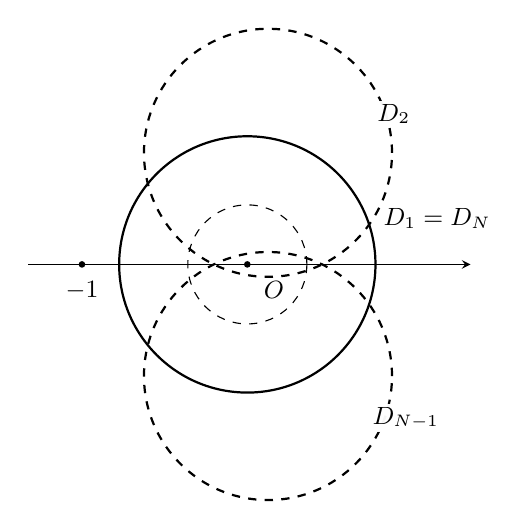
\begin{tikzpicture}[x=1.05cm,y=1.05cm,>=stealth,every node/.style={font=\small,fill=white,fill opacity=.96,text opacity=1,inner sep=1pt,outer sep=2pt}]
  \coordinate (B) at (-2.0,0);
  \coordinate (O) at (0,0);
  \draw[->] (-2.65,0)--(2.7,0);
  \draw[thick] (O) circle (1.55);
  \draw[dashed,thick] (0.25,1.35) circle (1.50);
  \draw[dashed,thick] (0.25,-1.35) circle (1.50);
  \draw[dashed] (0,0) circle (.72);
  \fill (B) circle (1.2pt) node[below=3pt] {$-1$};
  \fill (O) circle (1.2pt) node[below right=3pt] {$O$};
  \node[right=5pt] at (1.38,.56) {$D_1=D_N$};
  \node[right=4pt] at (1.34,1.82) {$D_2$};
  \node[right=4pt] at (1.28,-1.86) {$D_{N-1}$};
\end{tikzpicture}
\caption*{图3-4-2}
\end{figure}
在第二章中我们说，这个函数常被人们说成是多值函数，其实是黎曼曲面上的单值函数。所以，一个如(3)那样的幂级数，经过一切可能的解析延拓，将得到一个定义于其黎曼曲面上的单值函数。我们把这样得到的函数称为整体解析函数。

\noindent\textbf{定义2}\quad 从某一具有正收敛半径的幂级数(3)开始，经一切可能的解析延拓所得到的定义于其黎曼曲面上的函数称为一个整体的解析函数。

读者们可能会感到黎曼曲面是一个虽然有趣但是过于玄妙的东西。不过我们要问一问读者，我们生活于其中的空间当真是那么简单吗？20世纪下半叶的全部科学的发展都表明，空间是极为玄妙的，至今我们都说不清它的构造。所以，如果有朝一日发现黎曼曲面有深刻的物理意义，或者有助于说明这个深刻的物理问题，我们不必感到吃惊。

\subsection*{4. 柯西--黎曼方程、共形映射}

现在读者已经可以感到了，复变量函数的解析性是一个内涵非常丰富的概念。复变量函数 $w=f(z)$ 是从 $z$ 平面的开集（我们只考虑开集）$\Omega$ 到 $w$ 平面的映射，可是 $z$ 平面也就是 $\mathbb R^2$ 平面 $z=x+iy$，$w=u+iv$ 平面也就是另一个 $\mathbb R^2$ 平面：$(u,v)$ 平面，因此从几何上看 $w=f(z)$ 也是一个映射：$\Omega\subset\mathbb R^2\to\mathbb R^2$。而 $f(z)$ 的解析性的要求就包括了 $u$ 与 $v$ 在 $\Omega$ 中有连续的偏导数 $u_x,u_y,v_x,v_y$。$f'(z)$ 的存在说明当 $z+h$ 以任何方式趋向 $z$ 时，$\Delta f/\Delta z$ 当 $\Delta z=h\to0$ 时都有相同极限。现在我们看 $h=h_1+ih_2$，$h_1,h_2$ 为实数，以特定方式趋向0的后果。一是 $h_1=0,h_2\to0$，这时我们有
\[
\begin{aligned}
 \lim_{h\to0}\frac{\Delta f}{\Delta z}
 &=\lim_{h_2\to0}\left(
 \frac{u(x,y+h_2)-u(x,y)}{ih_2}
 +i\frac{v(x,y+h_2)-v(x,y)}{ih_2}\right)\\
 &=\frac1i\left(\frac{\partial u}{\partial y}+i\frac{\partial v}{\partial y}\right).
\end{aligned}
\]
同样，令 $h_2=0$，而 $h_1\to0$，这时我们有
\[
 \lim_{h\to0}\frac{\Delta f}{\Delta z}
 =\lim_{h_1\to0}\left(
 \frac{u(x+h_1,y)-u(x,y)}{h_1}
 +i\frac{v(x+h_1,y)-v(x,y)}{h_1}\right)
 =\frac{\partial u}{\partial x}+i\frac{\partial v}{\partial x}.
\]
比较这两个式子即得：$f'(z)$ 存在而且连续意味着 $u,v\in C^1(\Omega)$ 而且
\begin{equation}
 \frac{\partial u}{\partial x}=\frac{\partial v}{\partial y},\qquad
 \frac{\partial u}{\partial y}=-\frac{\partial v}{\partial x}.
 \tag{18}
\end{equation}
(18)式称为柯西--黎曼（Cauchy--Riemann，以下简称 C--R）方程组，或称为 C--R 条件。所以上面我们证明了若 $f(z)$ 是 $\Omega$ 中的解析函数，则必有 $f\in C^1(\Omega)$ 而且其实部虚部适合 C--R 条件。读者自己也容易证明其逆：若 $f(z)=u+iv$ 之实部虚部均为 $C^1(\Omega)$ 函数，而且适合 C--R 方程组，则 $f(z)$ 必是 $\Omega$ 中的解析函数，因为容易证明 $\lim_{\Delta z\to0}\Delta f/\Delta z$ 存在且连续，且
\[
 f'(z)=\frac{\partial u}{\partial x}+i\frac{\partial v}{\partial x}
 =-i\frac{\partial u}{\partial y}+\frac{\partial v}{\partial y}
\]
即是这个极限，所以也可以用 C--R 条件来作为解析性定义的基础。

上面我们把 $w=f(z)$ 看成是 $\Omega\subset\mathbb R^2\to\mathbb R^2$ 的一个映射，但这个映射一般并不是微分同胚。因为它的雅可比行列式
\begin{equation}
 J=\begin{vmatrix}u_x&u_y\\ v_x&v_y\end{vmatrix}
 =u_xv_y-u_yv_x=u_x^2+u_y^2=|f'(z)|^2
 \tag{19}
\end{equation}
可能在某些孤立点为0。我们来看当 $J\ne0$ 时这个映射的几何本质。在此映射下，线段 $(z,z+h)$ 的像是一曲线，这个线段与实轴的交角是 $\arg h$。按微分学的基本思想，其像在忽略了一个与 $|h|$ 比较为高阶的无穷小量之后，仍是直线，即过 $w=f(z)$ 点的切线（即图3-4-3之虚线）：
\[
 f(z+h)-f(z)=f'(z)h+o(h),\qquad\text{(曲线)}
\]
\[
 w=f(z)+f'(z)h,\qquad\text{(切线)}
\]
\begin{figure}[htbp]
\centering
\begin{tikzpicture}[x=.9cm,y=.9cm,>=stealth,every node/.style={font=\small,fill=white,fill opacity=.96,text opacity=1,inner sep=1pt,outer sep=2pt}]
  % z-plane
  \begin{scope}[shift={(-3.7,0)}]
    \draw[->] (-.2,0)--(4.2,0);
    \draw[->] (0,-.2)--(0,3.9);
    \node[above right] at (0,3.45) {$(z)$};
    \coordinate (Z) at (1.0,.6);
    \coordinate (H) at (3.05,2.6);
    \draw[thick] (Z)--(H);
    \draw[thick] (Z)--(2.08,3.35);
    \draw[dashed] (Z)--(3.2,.6);
    \fill (Z) circle (1.2pt) node[below left=3pt] {$z$};
    \fill (H) circle (1.2pt) node[right=3pt] {$z+h$};
    \draw[->] ($(Z)+(0.70,0)$) arc[start angle=0,end angle=44,radius=.70];
    \node at ($(Z)+(1.0,.33)$) {$\arg h$};
    \draw[->] ($(Z)+(0.53,.52)$) arc[start angle=44,end angle=69,radius=.74];
    \node at ($(Z)+(1.0,1.10)$) {$\alpha$};
  \end{scope}
  % w-plane
  \begin{scope}[shift={(3.4,0)}]
    \draw[->] (-.2,0)--(4.2,0);
    \draw[->] (0,-.2)--(0,3.9);
    \node[above right] at (0,3.45) {$(w)$};
    \coordinate (W) at (1.25,.62);
    \draw[dashed,thick] (W)--(2.12,3.45);
    \draw[thick] (W)--(3.15,2.18);
    \draw[thick] (W)--(.88,3.20);
    \draw[dashed] (W)--(3.3,.62);
    \fill (W) circle (1.2pt) node[below=4pt] {$w=f(z)$};
    \draw[->] ($(W)+(0.72,0)$) arc[start angle=0,end angle=40,radius=.72];
    \node[right=1pt] at ($(W)+(1.15,.35)$) {$\arg f'+\arg h$};
    \draw[->] ($(W)+(0.43,.48)$) arc[start angle=40,end angle=76,radius=.65];
    \node[left=1pt] at ($(W)+(.43,1.10)$) {$\alpha$};
  \end{scope}
\end{tikzpicture}
\caption*{图3-4-3}
\end{figure}
这条直线的倾角是
\[
 \arg f'(z)h=\arg f'(z)+\arg h.
\]
所以原线段 $(z,z+h)$ 之像，略去一个高阶无穷小量后，其方向是原直线段的方向再旋转一个角度 $\arg f'(z)$。在这里我们看到了 $f'(z)\ne0$ 这个条件的作用。因为若 $f'(z)=0$ 则 $\arg f'(z)$ 没有意义。若过 $z$ 点作另一条直线段而与原直线段交角为 $\alpha$，则它在映射 $w=f(z)$ 下之像，过 $f(z)$ 点的切线也将旋转一个角度 $\arg f'(z)$ 而与上一直线段之像的交角仍为 $\alpha$。总之，由复变量的解析函数 $w=f(z)$ 生成的映射在 $f'(z)\ne0$ 之处保持角度不变，所以称为共形映射（conformal mapping）。

这一种研究复变量的解析函数的几何方法始自黎曼，时为19世纪中叶。当时电磁学的问题正是整个物理科学的中心问题。我们可以从静电学的角度来看 C--R 条件的重要性。如果我们在平面上放上一些电荷，平面上原来已有的电场在放上电荷后将立即变化，而终于会达到一种稳态，即与时间无关的状态。这就是静电场。在此平面上取一个区域 $\Omega$，$\Omega$ 内的平面静电场可以用一个二维向量 $E$ 来表示：$E=(E_x,E_y)$，但是二维向量与复数是一回事，所以这个平面静电场可以用 $(x,y)$ 的复值函数 $E_x(x,y)+iE_y(x,y)$ 来表示。在静电场的情况应该存在电位 $u(x,y)$ 使
\begin{equation}
 E=\operatorname{grad}u,
 \tag{20}
\end{equation}
亦即
\begin{equation}
 E_x=\frac{\partial u}{\partial x},\qquad E_y=\frac{\partial u}{\partial y}.
 \tag{21}
\end{equation}
除了有电位 $u(x,y)$ 以外，还有一个重要的关系式如下：如果在 $\Omega$ 内没有电荷，则由高斯定理知应有
\begin{equation}
 \operatorname{div}E=\frac{\partial E_x}{\partial x}+\frac{\partial E_y}{\partial y}=0.
 \tag{22}
\end{equation}
现在我们要介绍一个重要定理。众所周知，对适当光滑的函数 $\varphi$，$\dfrac{\partial^2\varphi}{\partial x\partial y}=\dfrac{\partial^2\varphi}{\partial y\partial x}$，所以，如果上面的 $E_x$ 与 $-E_y$ 分别是某一函数 $v$ 的偏导数，则上式自然成立。这里有一个重要定理（庞加莱引理）若 $\Psi_1,\Psi_2$ 适合
\[
 \frac{\partial\Psi_2}{\partial x}=\frac{\partial\Psi_1}{\partial y},
\]
则它们一定是某个函数 $\varphi$ 的偏导数：$\Psi_1=\dfrac{\partial\varphi}{\partial x}$，$\Psi_2=\dfrac{\partial\varphi}{\partial y}$。这个结论的证明以及必须加上的条件将在第七章中详细讨论。将它用于 $E_x$ 与 $-E_y$ 即知，一定存在一个函数 $v(x,y)$ 使
\begin{equation}
 E_x=\frac{\partial v}{\partial y},\qquad -E_y=\frac{\partial v}{\partial x}.
 \tag{23}
\end{equation}
与(21)比较，即知 $u+iv$ 适合 C--R 条件。因此，再附上适当的光滑性要求即知解析函数是描述平面静电场的适合的数学工具。其实，类似的情况还不只出现在静电学中，例如18世纪的欧拉（还有18世纪的达朗贝尔）在流体力学中也遇到过它，所以 C--R 方程也称为欧拉--达朗贝尔方程，特别是我们容易看到，由 C--R 方程可得
\[
 \frac{\partial^2u}{\partial x^2}+\frac{\partial^2u}{\partial y^2}=0,
 \qquad
 \frac{\partial^2v}{\partial x^2}+\frac{\partial^2v}{\partial y^2}=0.
\]
即解析函数的实部虚部都适合拉普拉斯方程。而这是拉普拉斯在研究重力场的位势时得出的。

值得注意的是，本章§1讲的几个数学物理中的偏微分方程的导出都比较简单，利用守恒律——甚至傅里叶犯了一个错误，把热当成一种流质来看待时，也还是在利用守恒律，然后再略去高阶无穷小量即得。现在却不同了。两次利用了位势的存在——后面用庞加莱引理得出 $v$ 时，虽然 $v$ 的物理意义并不清楚，但和电位的存在十分相似，这不是牛顿的微分学所能概括的。比之后来的麦克斯韦方程来说，静电场的研究还只是最简单的一步。我们在这本书中，还要追随着整个数学的发展，最后看到用数学来刻画电磁现象（包括光学）时，整个数学的发展已经远远地超越了牛顿。

还是回到本章主题，有了微积分，把它推广到复域是最直接也是最重要的一大发展。我们就看到了复变量的解析函数的内容多么丰富。等到我们看到了复域中的积分学又给我们带来什么惊喜的时候，对这一发展之大就更有体会了。
